% Options for packages loaded elsewhere
\PassOptionsToPackage{unicode}{hyperref}
\PassOptionsToPackage{hyphens}{url}
%
\documentclass[
  9pt,
  ignorenonframetext,
]{beamer}
\usepackage{pgfpages}
\setbeamertemplate{caption}[numbered]
\setbeamertemplate{caption label separator}{: }
\setbeamercolor{caption name}{fg=normal text.fg}
\beamertemplatenavigationsymbolsempty
% Prevent slide breaks in the middle of a paragraph
\widowpenalties 1 10000
\raggedbottom
\setbeamertemplate{part page}{
  \centering
  \begin{beamercolorbox}[sep=16pt,center]{part title}
    \usebeamerfont{part title}\insertpart\par
  \end{beamercolorbox}
}
\setbeamertemplate{section page}{
  \centering
  \begin{beamercolorbox}[sep=12pt,center]{part title}
    \usebeamerfont{section title}\insertsection\par
  \end{beamercolorbox}
}
\setbeamertemplate{subsection page}{
  \centering
  \begin{beamercolorbox}[sep=8pt,center]{part title}
    \usebeamerfont{subsection title}\insertsubsection\par
  \end{beamercolorbox}
}
\AtBeginPart{
  \frame{\partpage}
}
\AtBeginSection{
  \ifbibliography
  \else
    \frame{\sectionpage}
  \fi
}
\AtBeginSubsection{
  \frame{\subsectionpage}
}
\usepackage{lmodern}
\usepackage{amsmath}
\usepackage{ifxetex,ifluatex}
\ifnum 0\ifxetex 1\fi\ifluatex 1\fi=0 % if pdftex
  \usepackage[T1]{fontenc}
  \usepackage[utf8]{inputenc}
  \usepackage{textcomp} % provide euro and other symbols
  \usepackage{amssymb}
\else % if luatex or xetex
  \usepackage{unicode-math}
  \defaultfontfeatures{Scale=MatchLowercase}
  \defaultfontfeatures[\rmfamily]{Ligatures=TeX,Scale=1}
\fi
\usetheme[]{Goettingen}
\usecolortheme{rose}
% Use upquote if available, for straight quotes in verbatim environments
\IfFileExists{upquote.sty}{\usepackage{upquote}}{}
\IfFileExists{microtype.sty}{% use microtype if available
  \usepackage[]{microtype}
  \UseMicrotypeSet[protrusion]{basicmath} % disable protrusion for tt fonts
}{}
\makeatletter
\@ifundefined{KOMAClassName}{% if non-KOMA class
  \IfFileExists{parskip.sty}{%
    \usepackage{parskip}
  }{% else
    \setlength{\parindent}{0pt}
    \setlength{\parskip}{6pt plus 2pt minus 1pt}}
}{% if KOMA class
  \KOMAoptions{parskip=half}}
\makeatother
\usepackage{xcolor}
\IfFileExists{xurl.sty}{\usepackage{xurl}}{} % add URL line breaks if available
\IfFileExists{bookmark.sty}{\usepackage{bookmark}}{\usepackage{hyperref}}
\hypersetup{
  pdftitle={BIOS6643 Longitudinal},
  pdfauthor={EJC},
  hidelinks,
  pdfcreator={LaTeX via pandoc}}
\urlstyle{same} % disable monospaced font for URLs
\newif\ifbibliography
\setlength{\emergencystretch}{3em} % prevent overfull lines
\providecommand{\tightlist}{%
  \setlength{\itemsep}{0pt}\setlength{\parskip}{0pt}}
\setcounter{secnumdepth}{-\maxdimen} % remove section numbering
\AtBeginSubsection{}
\AtBeginSection{}
\ifluatex
  \usepackage{selnolig}  % disable illegal ligatures
\fi

\title{BIOS6643 Longitudinal}
\subtitle{L20 Missing data}
\author{EJC}
\date{}
\institute{Department of Biostatistics \& Informatics}

\begin{document}
\frame{\titlepage}

\begin{frame}[allowframebreaks]
  \tableofcontents[hideallsubsections]
\end{frame}
\hypertarget{interpretation}{%
\section{Interpretation}\label{interpretation}}

\begin{frame}{Topics for today}
\protect\hypertarget{topics-for-today}{}
Time-varying age versus baseline age in longitudinal data analyses

Separating within and between-subject effects for time-varying
covariates

Measuring the relationship between a time-varying covariate and an
outcome for longitudinal data

Modeling time as a class or continuous variable

Population-averaged versus subject-specific effects

\vspace{\baselineskip}

\textbf{Related reading: Interpreting parameters in longitudinal models
course notes}
\end{frame}

\begin{frame}{Time-varying age versus baseline age in longitudinal data
analyses}
\protect\hypertarget{time-varying-age-versus-baseline-age-in-longitudinal-data-analyses}{}
Most longitudinal experiments and studies involve a relatively short
amount of time, anywhere from a few weeks to a few months. Typically
there is a time variable to indicate when measurements were taken.

If one is interested in also including age of subjects as a covariate
into the model, typically baseline age is used - i.e., the fixed age for
subjects when they enter the study. But one question that arises is,
should a time-varying age be used, or baseline age?

Many think that baseline age is most appropriate when another time
variable is already in the model. Here, we will examine both approaches
mathematically, and the results may surprise you a little bit, although
we will also see that you can easily estimate effects of interest from
either approach.
\end{frame}

\begin{frame}{}
\protect\hypertarget{section}{}
Consider a study in which subjects' blood pressures are observed over
time (3 time points, equally spaced, no missing data). The model will
include fixed effects for time, age (at start of experiment) and gender;
and a random intercept for subjects. The AR(1) structure will be used to
model the errors. In the model, age at start of experiment (i.e.,
baseline) was used. How would estimates change if you used continuous
age in the model instead?

In order to answer the question, write out the statistical models for
both approaches. Note that \(real_{age} = BL_{age} + time\). Thus, the
model using real age (but not including gender) is

\(E[Y]= \beta_0+ \beta_1 real_{age}+ \beta_2 time\)\\
\(E[Y]= \beta_0+ \beta_1 (BL_{age} +time)+ \beta_2 time\)\\
\(E[Y]= \beta_0+ \beta_1 BL_{age}+( \beta_1+ \beta_2)time\)\\
\(E[Y]= \beta_0+ \beta_1 BL_{age}+ \beta_2^{new} time\)

So we have expressed the model with real age in terms of the one that
uses baseline age. Thus, the underlying models are the same. However,
the interpretation of the parameters differs for the 2 approaches, as
the above equations suggest.
\end{frame}

\begin{frame}{}
\protect\hypertarget{section-1}{}
Considering the models above, \(\beta_1\) is a between-subject age
effect, regardless of whether \(real_{age}\) or \(BL_{age}\) is used;
\(\beta_2\) is a within-subject time (or age) effect; \(\beta_2^{new}\)
is the combination of these. So in order to get effects of time that
does not involve between-subject age effects, we use the model with
\(real_{age}\).

As an example of when this may be of interest; the Beryllium natural
history project involved evaluating the progression of illness that was
not due to the aging process (specifically, we removed between-subject
age effects from the time variable). Thus, real age was used in the
analysis.

In many other cases, \(BL_{age}\) is used, although many probably don't
really understand the difference between the two approaches. But often
there won't be a great difference unless the study is over a longer
period of time. You can estimate all parameters mentioned above from
either model (e.g., by including an appropriate ESTIMATE statement in
PROC MIXED).
\end{frame}

\hypertarget{separating-within-and-between-subject-effects-for-time-varying-covariates}{%
\section{Separating within and between-subject effects for time-varying
covariates}\label{separating-within-and-between-subject-effects-for-time-varying-covariates}}

\begin{frame}{Methods and simpler models}
\protect\hypertarget{methods-and-simpler-models}{}
Data from many longitudinal experiments or studies are fit in
regression-type models (e.g., mixed models), where each time-varying
covariate is fit with one term. For example, in the Kunsberg / air
pollution studies that I've been involved with, we fit health outcome
models as a function of an air pollution variable (with a fixed-effect
coefficient) plus other fixed and random effect terms. When personal
monitors are used, the pollution variable is both subject and
time-specific (i.e., subject-varying and time-varying).

If just one term is used for the pollution variable, then we are fitting
a parameter that involves pooled effects based on between-subjects
differences as well as within-subject changes over time. To illustrate,
consider a linear mixed model with a random intercept for subjects and
fixed-effect term(s) for pollutant variable(s). Here, \(Y_{ij}\) is some
health outcome measure such as FEV1 and say \(x_{ij}\) is the
subject-specific (i.e., personal) pollution level for subject \(i\) on
day \(j\): \(Y_{ij}= \beta_0+b_{0i}+\beta x_{ij}+\epsilon _{ij}\) For
subject \(i\), \(Y\) changes by an expected amount
\(\beta (x_{ij}-x_{i'j})\) from day \(j\) to \(jʹ\). Similarly, for day
\(j\), the expected difference between subject \(i\) and \(iʹ\) is
\(\beta (x_{ij}-x_{i'j})\). The within and between-subject effects get
pooled as there is only one slope parameter for the pollutant variable.
We can obtain separate estimates for between-subject and within-subject
effects. To do this, note that \(x_{ij}=\bar x_i+(x_{ij}-\bar x_i)\).
\end{frame}

\begin{frame}{}
\protect\hypertarget{section-2}{}
Thus, by fitting terms separately for \(\bar x_i\) and
\(x_{ij}-\bar x_i\), we can determine if slope estimates differ for
within and between- subject data. If there is no difference, then it is
not necessary to use the separate terms. {[}You could also use
\(\bar x_i\) and \(x_{ij}\) as the BS and WS variables, respectively.
What are the implications?{]}

To further illustrate, consider a study where birth weight is the
outcome for 880 mothers that had 5 children (data from CDC), and the
time-varying covariate is the mother's age at each birth (denoted by
\(x_{ij}\), where \(i\) indexes subject, \(i=1,\ ...,\ 880\), and \(j\)
indexes the birth event \(j=1,\ ...,\ 5\)).
\end{frame}

\begin{frame}{}
\protect\hypertarget{section-3}{}
Here are the models:

\(Y_{ij}= \beta_0+b_{0i}+\beta x_{ij}+\epsilon _{ij} \ \ \ \ (1)\)\\
\(Y_{ij}= \beta_0+b_{0i}+ \beta_B \bar x_i+ \beta_W (x_{ij}-\bar x_i)+\epsilon _{ij} \ \ \ \ (2)\)

where \(\epsilon _{ij}\sim \mathcal N(0,\ \sigma_\epsilon ^2)\),
\(b_{i0}\sim \mathcal N(0,\ \sigma_b^2)\) for both models.

Fitting model (1) yields \(\hat \beta=17.14\) grams, which indicates
that increase in birth weight increases is about 17 grams, on average,
per year.

However, when model (2) is fit, we obtain \(\hat \beta_B=30.35\) grams
and \(\hat \beta_W=11.83\) grams.

We would estimate that average birth weight will differ by about 30
grams between two women whose average birth age differs by one year.

For a given woman, we would estimate that the birth weights of her
children increase by an average of about 11.8 grams for each year that
she ages.
\end{frame}

\begin{frame}{}
\protect\hypertarget{section-4}{}
The increase estimates here may be largely due to the fact that younger
women were studied - the median age at first birth was 17 years! For
more detail, see Neuhaus and Kalbfleisch, \textbf{Between and
within-cluster covariate effects in the analysis of clustered data}.
Biometrics, 54, 638-645, 1998. Hedeker also discusses this issue on
pages 72-74.

Below are predicted values for subjects (blue) and the between-subject
average fit (red) for a random sample of the 878 mothers.

\begin{center}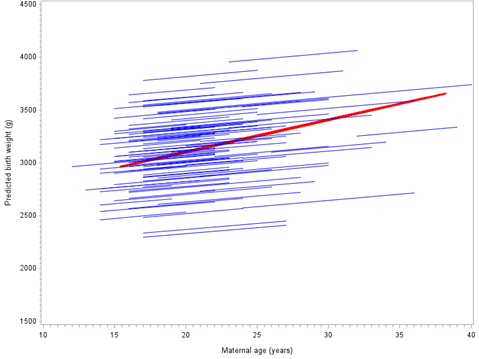
\includegraphics[width=0.7\linewidth]{figs_L19/f1} \end{center}
\end{frame}

\begin{frame}{Case study: More advanced models with Bolder Boulder data}
\protect\hypertarget{case-study-more-advanced-models-with-bolder-boulder-data}{}
The Bolder Boulder is a 10K race held in Boulder, Colorado on Memorial
Day. The race has been run for several decades, and is one of the
largest running races in the United States. Using this data, we can
estimate between and within-subject changes over time. However, modeling
these data requires nonlinear functions, (see \textbf{Non-normal and
nonlinear notes}).

Here we consider 12 consecutive years of data where subjects may
participate in multiple years, and thus longitudinal data. In our
analysis we focused on the most competitive runners in the Citizen's
(nonprofessional) race. For more specifics on subject and record
inclusion, see the course notes.
\end{frame}

\begin{frame}{}
\protect\hypertarget{section-5}{}
The following figure shows a spaghetti plot of a random 20\% of runners,
for both men and women.

\begin{center}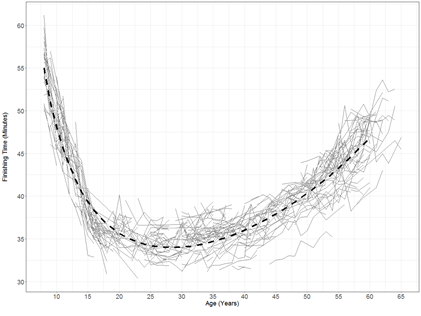
\includegraphics[width=0.4\linewidth]{figs_L19/f2} \end{center}

\begin{center}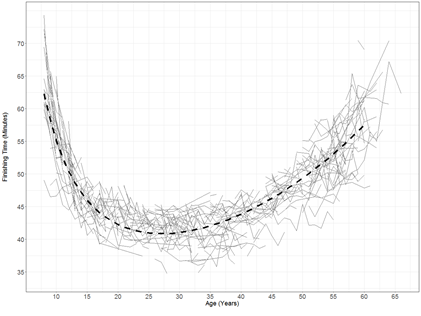
\includegraphics[width=0.4\linewidth]{figs_L19/f3} \end{center}

The function we use to model race time versus age is
\(f(x)=e^{\alpha _0 } x^{\alpha _1 } e^{\alpha _2x }\), however we can
linearize the function by taking natural logs of both sides:
\(ln⁡[f(x)]=\alpha _0+\alpha _1 ln⁡(x)+\alpha _2 x\).
\end{frame}

\begin{frame}{}
\protect\hypertarget{section-6}{}
This is important when separating effects into between-subject (BS) and
within-subject (WS) components, since the model will already be pretty
complex. Extending N \& K's idea of separating time-varying covariates
into between and within-subject components, we recognize that
\(x_{ij}=\bar x_i \Big(\frac {x_{ij}} {x_i} \Big)\). Thus we can write a
longitudinal nonlinear model that allows for both within and
between-subject effects, plus random effects for subjects:
\(Y_{ij}=e^{\alpha _0 } e^{b_{0i}} \bar x_i^{\alpha _1^B } \Big(\frac {x_{ij}} {\bar x_{i.}} \Big)^{\alpha _1^W+b_{1i}} e^{\alpha _2^B \bar x_i } e^{(\alpha _2^W+b_{2i})(x_{ij}- \bar x_{i.})} e^{\epsilon_{ij}}\)

where \(Y\) is the natural log race time, \(x\) is age, \(i\) indexes
subject and \(j\) time, and
\(\pmb b_i=(b_{0i},b_{1i},b_{2i})^{\top} \sim \mathcal N(\pmb 0,\ \pmb \Sigma)\),
independently of
\(\epsilon_{ij} \stackrel {iid} \sim N(0,\ \sigma_\epsilon ^2)\).

The log version, which is linear with respect to the parameters, is
\(lnY_{ij}=\alpha _0+\alpha _1^B ln(\bar x_i)+\alpha _2^B \bar x_i+b_{0i} +(\alpha _1^W+b_{1i})ln\Big(\frac {x_{ij}} {\bar x_{i.}}\Big)+(\alpha _2^W+b_{2i})(x_{ij}-\bar x_i)+\epsilon_{ij}\),
which is fit easily using standard LMM methods.
\end{frame}

\begin{frame}{}
\protect\hypertarget{section-7}{}
In order to get subject predicted values, we note that
\(E[Y_{ij}│\pmb b_i]= E[e^{\epsilon _{ij} }]e^{E[lnY_{ij}│\pmb b_i]}\).

The between-subject function is defined to be
\(E[Y_{ij}│\pmb b_i=0] |_{(x_{ij}=x_{i.})}=\alpha _0^B \bar x_i^{\alpha _1^B} e^{\alpha _2^B \bar x_i}\),
and the (average) within-subject function is
\(E[Y_{ij}│b_i=0]=\alpha _{0,\ \bar x_i.}^W x_{ij}^{\alpha_1^W} e^{\alpha_2^W} e^{\alpha _2^W x_{ij}}\)

where
\(\alpha _{0,\ x_{i.}}^W=e^{\alpha _0 } e^{0.5\sigma_\epsilon ^2} \bar x_{i.}^{\alpha _1^B-\alpha _1^W} e^{\bar x_{i.} (\alpha _1^B-\alpha _1^W)}\).
So this function can be constructed for a specific subject that has
average race age \(x_i\). (for those races satisfying the inclusion
criteria). As before, if the log version of the model is fit, we just
need to multiply exponentiated values by
\(E[e^{\epsilon_{ij}}]=e^{0.5\sigma_\epsilon ^2}\) in order to estimate
average values on the original scale.
\end{frame}

\begin{frame}{}
\protect\hypertarget{section-8}{}
The figures below show the estimated between and within-subject
funcitons for men and women (5 WS functions shown). The results
generally indicate that within changes generally occur a bit more slowly
than differences between subjects, particularly after the peak age and
more so for women.

\begin{center}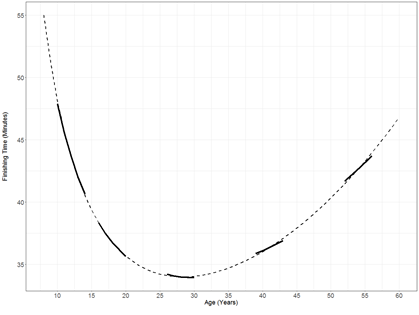
\includegraphics[width=0.4\linewidth]{figs_L19/f4} \end{center}

\begin{center}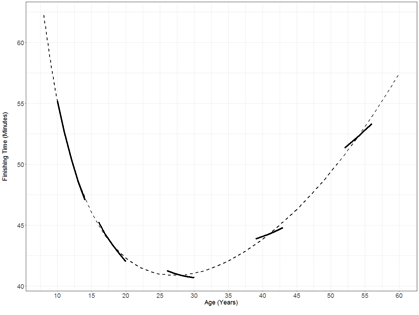
\includegraphics[width=0.4\linewidth]{figs_L19/f5} \end{center}
\end{frame}

\begin{frame}{}
\protect\hypertarget{section-9}{}
Using the between and within subject functions, we can better understand
how people change in performance over time.

\begin{itemize}
\item
  Using the BS function to find `peak age'
\item
  Rates of change in BS function: \textasciitilde{} 1\% per year decline
  at age 40, \textasciitilde{} 2\% per year at age 60. \emph{``A
  42-year-old male has an expected 1.0\% slower time than a 41-year-old
  (based on the between-subject curve)''}
\item
  Within-subject changes are a bit more attenuated relative to the
  between-subject curve. \emph{``A 41-year-old that participates in the
  following year is expected to only slow by a rate of 0.3\% based on
  the within-subject function.''}
\item
  For women, there is an even greater difference between BS and WS
  curves, as the graph displays.
\end{itemize}
\end{frame}

\hypertarget{modeling-time-as-a-class-or-continuous-variable}{%
\section{Modeling time as a class or continuous
variable}\label{modeling-time-as-a-class-or-continuous-variable}}

\begin{frame}{Modeling time as a class or continuous variable}
\protect\hypertarget{modeling-time-as-a-class-or-continuous-variable-1}{}
\begin{block}{Pro's and con's of approaches}
\protect\hypertarget{pros-and-cons-of-approaches}{}
For some data, it is pretty clear whether time should be modeled as a
class or continuous variable. For other data, it is not so clear.

If data involves 4 or 5 time points or less, modeling time as a class
variable typically yields a better fit. A wrinkle with this occurs when
actual times of measurement do not meet the prescribed dates (e.g., for
a `1-year' follow up, subjects might come in early or late). This has
happened in several student projects. Whether the time as class variable
should be abandoned really depends on the data and the degree of `error'
in times of measurement of subjects. If subjects still come in fairly
close to the prescribed dates then the class variable approach may still
provide a reasonable approximation.
\end{block}
\end{frame}

\begin{frame}{Inference when time is modeled as a continuous variable}
\protect\hypertarget{inference-when-time-is-modeled-as-a-continuous-variable}{}
We thoroughly examined tests involving \(group\), \(time\) and
\(group \times time\) terms when time was a class variable. When time is
modeled as a continuous variable, often the focus is more on estimation
and features of function being estimated (e.g., slope of a linear
function, minimum or maximum of a quadratic function, derivative of a
curve, etc.). In order to get the minimum or maximum of a parabola, you
can take the derivative of the fitted function, set it to 0 and solve
for \(x\). As an example, see the Non-normal notes and the Bolder
Boulder data application.

When there is a group variable and time is modeled as a continuous
variable, you can still easily perform hypothesis tests to compare
groups at particular time points (e.g., perform t-tests by including
ESTIMATE statements in PROC GLM or PROC MIXED to compare genders at
fixed ages since there is one degree of freedom for such tests). Some
examples are shown ahead.
\end{frame}

\begin{frame}{}
\protect\hypertarget{section-10}{}
Say you have two groups that you want to compare more generally. Here
are some possible tests of interest:

\begin{itemize}
\item
  Compare curves
\item
  Compare differences in curves over time minus intercept differences
  (i.e., interaction)
\item
  Compare highest order trend (e.g., compare quadratic trends if model
  is specified up through quadratic)
\end{itemize}

To determine how to write these tests, consider the model for the Mt.
Kilimanjaro data:
\(E[Y_{hij}]= \beta_0+ \beta_1 x_{ij}+ \beta_2 x_i^2+\alpha _h+\gamma _{h1} x_{ij}+\gamma _{h2} x_{ij}^2\),

where \(h\) indexes drug group, \(i\) indexes subject and \(j\) indexes
the repeated measure. (We don't need an `h' index on \(x\) as long as
the subject index is unique, study wide.) There is a similar model for
the Bolder Boulder data in the course notes \ldots{}
\end{frame}

\begin{frame}{}
\protect\hypertarget{section-11}{}
Below are the models expressed by Diamox users (never=0, ever=1)

Never users:
\(E[Y_{1ij}]=( \beta_0+\alpha _1)+( \beta_1+\gamma_{11})x_{ij}+( \beta_2+\gamma _{12})x_{ij}^2\)\\
Ever users:
\(E[Y_{2ij}]=( \beta_0+\alpha _2)+( \beta_1+\gamma_{21})x_{ij}+( \beta_2+\gamma _{22})x_{ij}^2\)

If the highest levels are set to 0 or if the SAS g-inverse is used,
then\\
\(\alpha _2=0,\gamma _{21} =0,\gamma _{22} =0\) and
\(\alpha _1,\gamma _{11} ,\gamma _{12}\) represent deviations of the
never-user function from the ever users, for intercept, linear and
quadratic terms, respectively. In this case, the ever-user function is
\(E[Y_{2ij}]= \beta_0+ \beta_1 x_{ij}+ \beta_2 x_{ij}^2\) .

For the LTFR model, the overall test to compare curves can be written as
\(H_0:\ \alpha _1-\alpha _2=0,\ \gamma _{11} -\gamma _{21} =0,\ \gamma _{12} -\gamma _{22} =0\).

Similarly, the interaction test is
\(H_0: \gamma _{11} -\gamma _{21} =0,\ \gamma _{12} -\gamma _{22} =0\).
\end{frame}

\begin{frame}{}
\protect\hypertarget{section-12}{}
The comma is important to separate rows; if you don't have a comma, then
the test (for interaction) becomes:
\(H_0: (\gamma _11-\gamma _21)+(\gamma _12-\gamma _22)=0\). This test is
probably not of interest, since you could have offsetting non-zero
values for the linear and quadratic differences. Next is the Mt.
Kilimanjaro data to show how such tests could be conducted using
\(F\)-tests (via CONTRAST statements), plus some simpler comparisons at
specific time points using ESTIMATE statements.

See previous slides for various models fit; the model here includes an
AR(1) structure for the errors in addition to random effects. Recall we
actually found an improved error covariance structure using the
Kronecker Product (using AM/PM and Day as two time components).
\end{frame}

\begin{frame}{}
\protect\hypertarget{section-13}{}
Recall also that `\(x\)' is altitude.

\begin{center}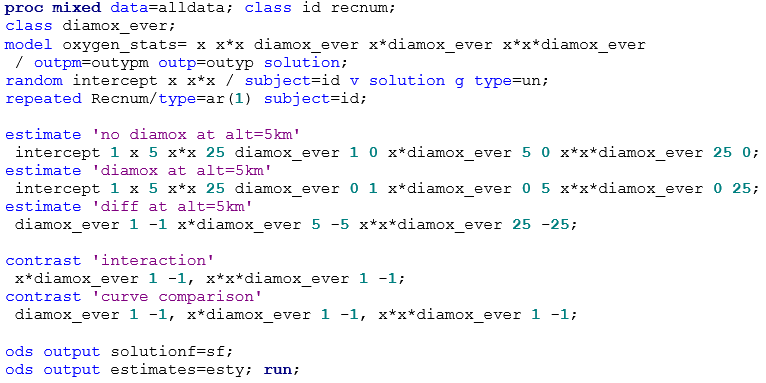
\includegraphics[width=0.7\linewidth]{figs_L19/f6} \end{center}

Review (for a snickers): In the CONTRAST statements above, what is the
difference between including and excluding the `,' between terms?
\end{frame}

\begin{frame}{Output:}
\protect\hypertarget{output}{}
\begin{center}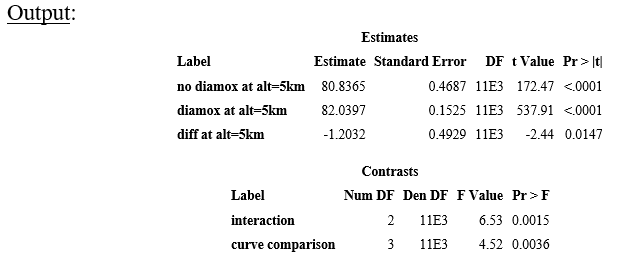
\includegraphics[width=0.7\linewidth]{figs_L19/f7} \end{center}

You can also create a model using diamox\_ever as a binary `continuous'
variable (i.e., do not include in the CLASS statement, but levels must
be 0 and 1), and obtain the same results. In this case only 1 column is
added to the \(X\) matrix and there is only 1 coefficient for
diamox\_ever instead of 2 (when writing contrasts and estimate
statements). Can you rewrite the ESTIMATE and CONTRAST statements in
this case?
\end{frame}

\begin{frame}{}
\protect\hypertarget{section-14}{}
The tests for individual coefficients of the \(group \times time\) and
\(group \times time2\) terms are probably less meaningful. These tests
are not like the polynomial interaction tests we considered when time
was modeled as a class variable.

When there are polynomial functions that differ by groups, tests at one
specific time point, or changes between time points may be of interest.

If applicable, so you also evaluate derivatives of functions to express
rate of change. If you have a quadratic function, the derivative
function expressing rate of change will be linear.

\begin{block}{Notes on DDF calculations}
\protect\hypertarget{notes-on-ddf-calculations}{}
In our case, the default method to calculate DDF for our custom t and F
tests is the `containment' method. For these data, the calculated DDF is
equal to the number of records used to fit the model (13369), minus the
number of random effect terms per subject times the number of subjects
(3*916=2748), so the DF is 13369 - 2748 = 10621. In the output, we just
see 11E3 but I used ODS OUTPUT to get the exact number.

If we use the RESIDUAL method, we essentially ignore the repeated
measures and treat each record as if it came from a different subject.
This would yield DDF=\(n-rank(\pmb X)\)=13369 - 6=13363.
\end{block}
\end{frame}

\begin{frame}{Population-averaged versus subject-specific effects}
\protect\hypertarget{population-averaged-versus-subject-specific-effects}{}
Beta parameters may have subject-specific or population-averaged
interpretations, depending on the type of model being fit. For Normal
outcomes, the interpretation is the same (which is why we have not
discussed this issue yet). But for some other types of outcomes, this
may not be so.

Consider a linear mixed model with random intercept and slope for time
(\(x\)), by subject, and fixed effects that also include an intercept
and slope for time (for simplicity we won't consider other covariates).

\begin{itemize}
\item
  The (estimated) population mean function is
  \(E[Y_{ij}]= \beta_0+ \beta_1 x_{ij}\).
\item
  The subject-specific function is
  \(E[Y_{ij} |b_i]= \beta_0+ \beta_1 x_{ij}+b_{0i}+b_{1i} x_{ij}\). In
  particular, the `average' subject has no deviation from the population
  average ( \(b_0\) and \(b_1\) are 0), and thus the mean is
  \(E[Y_{ij} |b_i=0]= \beta_0+ \beta_1 x_{ij}\).
\end{itemize}

Since the population average function is equivalent to the subject
specific function (for the average subject), we say that fixed effects
in this case have both population-averaged and subject-specific
interpretations. For other distributions, these may not be equal.
\end{frame}

\begin{frame}{}
\protect\hypertarget{section-15}{}
Consider a GzLMM where the outcome has a Poisson distribution, the fixed
effects include a simple linear trend for time, and there is a random
intercept for subjects: \(g(\mu_{ij}) = \beta_0+ \beta_1 x_{ij}+b_i\).

The conditional mean is
\(E[Y_{ij} |b_i=0]=e^{\beta_0+ \beta_1 x_{ij}}\); The marginal mean is
\(E[Y_{ij}]=E\big[E[Y_{ij}|b_i]\big]=E[e^{\beta_0+ \beta_1 x_{ij}+b_i}]=e^{\beta_0+0.5 \sigma_b^2} e^{\beta_1 x_{ij}}=e^{ \beta_0'} e^{\beta_1 x_{ij}}\)

The only difference between these means is in the intercept; it is
greater in the marginal mean by the amount \(0.5 \sigma_b^2\) compared
with the conditional mean (for subjects with \(b_i=0\)). The parameter
\(\beta_1\) is typically of more interest and has both specific-subject
and population-averaged interpretations. However, results do not
necessarily generalize for more complex random effects.

For a binary outcome, \(\beta_1\) will have different interpretations,
considering the model \(g(\mu_{ij}) = \beta_0+ \beta_1 x_{ij}+b_i\),
where \(g\) is the logit link.
\end{frame}

\begin{frame}{}
\protect\hypertarget{section-16}{}
The graph below shows \(E[Y_{ij}]\), red, with subject curves,
\(E[Y_{ij} |b_i]\), black. {[}\(E[Y_{ij} |b_i=0]\) is solid and the rest
are dashed.{]} \emph{Clearly the population averaged function (solid
red) is not the same as the function for the average subject (solid
black)}. Importantly, the slope of the marginal mean function is flatter
(more attenuated) compared with the conditional mean function.

\begin{center}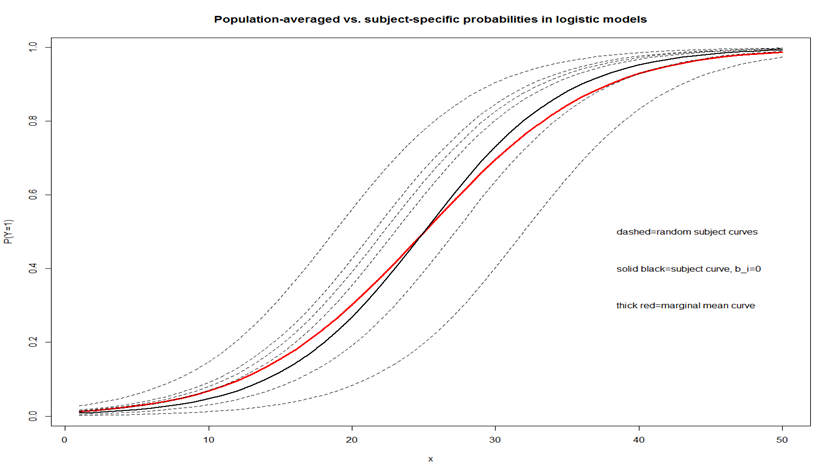
\includegraphics[width=0.7\linewidth]{figs_L19/f8} \end{center}
\end{frame}

\begin{frame}{Implications}
\protect\hypertarget{implications}{}
For populations where there is subject heterogeneity (e.g., random
intercept differences):

\begin{itemize}
\item
  Using GzLM/GEE will yield beta estimates that have population-averaged
  (PA) interpretations.
\item
  Using GzLMM's with the appropriate random effect terms will yield beta
  estimates that have subject-specific (SS) interpretations.
\end{itemize}

In some cases (normal theory models, some effects in some Poisson
models), they are one in the same.

We also learned that estimates based on the pseudo-likelihood approach
for GzLMM can be subject-specific or population-averaged, depending on
whether random-effect estimates are include in the Taylor series
expansion or not (see GzLMM linearization slides).
\end{frame}

\hypertarget{summary}{%
\section{Summary}\label{summary}}

\begin{frame}{Summary}
\protect\hypertarget{summary-1}{}
A predictor that varies over subjects and time can be split into 2
components, and separate coefficients given in order to estimate
between-subject and within-subject effects; otherwise, the effect being
estimated pools the BS and WS effects.

For complex models used with longitudinal data (e.g., mixture models,
BS/WS models or other nonlinear models), random effects can be `added
to' parameters to get subject-specific predicted values.

To understand disease progression, you may want to consider including
time-varying age in the model, even if a separate time variable is also
included. This way, aging effects are more clearly separated from
disease progression effects.
\end{frame}

\begin{frame}{}
\protect\hypertarget{section-17}{}
Consider binary longitudinal data with subject heterogeneity, where
logistic regression is used to model the data.

\begin{itemize}
\item
  Beta parameters of predictors in GEE models will have
  population-averaged interpretations; the subject heterogeneity gets
  embedded into the marginal mean that averages over subjects; this
  `flattens' the S-curve (beta is attenuated).
\item
  Beta parameters of predictors in GzLMM models have subject-specific
  interpretations (if the random intercept is included). Here instead
  averaging functions over subjects (as the marginal mean does), we
  determine the (mean) function for the average subject. (See graph.)
\item
  The PA function does not represent any one subject in the population;
  the SS function represents every subject (in terms of slope); they are
  just shifted by random intercept amounts.
\item
  In practice, there may not be much difference between the two
  approaches, it depends on the application. The more the subject
  heterogeneity (higher the variance), the bigger the potential
  difference.
\end{itemize}
\end{frame}

\end{document}
